% See author's guidelines for Methods in Ecology and Evolution:
% http://www.methodsinecologyandevolution.org/view/0/authorGuidelines.html

\documentclass[12pt]{article}

% One-inch margins
\usepackage{fullpage}

% No orphans or widows
\usepackage[all]{nowidow}

% Additional math features
\usepackage{amsmath}

% Use mee bibliography style
\usepackage{natbib}
\bibliographystyle{mee}

% Include figures
\usepackage{graphicx}

% Definitions to make it easier to type
\newcommand{\MCMCMC}{(MC)$^{3}$}
\newcommand{\MCMCMCMC}{(MC)$^{4}$}

\begin{document}

% Double-spaced
\baselineskip 24pt

\begin{flushleft}

{\Large\textbf{Multi-core Metropolis coupled Markov chain Monte Carlo
    for detecting rate shifts on phylogenetic trees using BAMM}}

% Short title must be <= 45 characters (current: 47, including spaces)
\textbf{Short title:} Metropolis coupled MCMC for rate shift detection

% Recommended: 6000-7000 words, including tables, figure captions, references
\textbf{Word count:} 3,218

Carlos J. R. Anderson$^{1}$ and
Daniel L. Rabosky$^{1,*}$

$^{1}$Department of Ecology and Evolutionary Biology,
    University of Michigan, Ann Arbor, MI 48109, USA

$^{*}$Corresponding author: Daniel L. Rabosky (drabosky@umich.edu)

\end{flushleft}


\pagebreak[4]


% Maximum of 350 words
\section*{Abstract}

% Suppress indentation for the following paragraphs
{\setlength{\parindent}{0cm}

\textbf{1.}
BAMM (Bayesian Analysis of Macroevolutionary Mixtures) is a computer program
that uses Markov chain Monte Carlo (MCMC) to model complex dynamics
of speciation, extinction, and trait evolution on phylogenetic trees.
%
Previous versions of BAMM used a single Markov chain
to explore the landscape of models and their parameter values.
%
A single chain, however, may get stuck in local optima,
resulting in poor performance in both mixing and convergence.

\textbf{2.}
Here we describe an extension to BAMM
that implements Metropolis coupled MCMC [\MCMCMC].
%
With \MCMCMC, additional chains are introduced
that are able to explore more of the model landscape.
%
Swaps between chains may occur periodically,
so if a chain is stuck in a local optimum,
it may immediately jump to another area of the landscape.
%
In addition, we describe multi-core \MCMCMC\ [\MCMCMCMC]
which runs each chain on a separate computer processor.

\textbf{3.}
Using both simulated phylogenetic trees and an empirical tree,
we find that runs with \MCMCMC\ mix better than those with a single chain.
%
In simulated trees, convergence in runs with or without \MCMCMC\ 
is about the same, but in the skink tree,
convergence is better in runs with \MCMCMC\ than those without.
%
\MCMCMCMC\ speeds up the run times close to $n$-fold
for runs with $n$ chains.

\textbf{4.}
\MCMCMC\ and \MCMCMCMC\ greatly improve
the efficiency and speed of runs in BAMM,
and we recommend their use in future studies of macroevolutionary dynamics.
}

\begin{flushleft}
\textbf{Key-words:} BAMM, Bayesian, macroevolution, phylogeny, skink, speciation
\end{flushleft}


\pagebreak[4]


% State the reason for the work, the context and the hypotheses being tested
\section*{Introduction}

\subsection*{Background}

The variation in species richness and phenotypic diversity we see today
across groups of organisms is partly due to the stochastic
evolutionary processes of speciation and extinction \citep{rab14plos}.
%
Rates of speciation and extinction differ among groups
and have changed through time as a result of unique historical events,
such as environmental, phenotypic, and genetic changes.
%
For example, speciation could dramatically increase
during an adaptive radiation of a species on a newly colonized island.
%
Consequently, the phenotypic diversity of this colonizing group
would also increase as organisms adapt and fill
the available ecological niches.


The processes of speciation and extinction within a group of organisms
have shaped the topology of their phylogenetic tree.
%
Phylogenetic trees can therefore be used to extract
information about the complex dynamics that shaped them \citep{rab14plos}.
%
For example, an adaptive radiation would show up
as a burst in the number of splits and branches on a tree.
%
In addition, a phylogenetic tree would likely be composed of several processes,
each with a unique rate of diversification or morphological evolution.
%
A new method was recently developed to identify and characterize
such macroevolutionary processes across phylogenetic trees \citep{rab14plos}.


\subsection*{BAMM}

BAMM (Bayesian Analysis of Macroevolutionary Mixtures)
is a computer program that searches for models that best explain
the complex dynamics of evolutionary processes on phylogenetic trees.
%
For speciation dynamics, a process is defined as the rate of speciation
modeled as an exponential function through time.
%
A process may occur on any branch of a tree,
and all branches downstream of the process are under its control.
%
There may be multiple processes on a tree,
and each process can have its own set of parameters.
%
Processes may be nested, where a process may occur
within a clade controlled by another process.
%
In such a case, the process downstream of the ``ancestral'' process
takes over the dynamics of the branches downstream of it.


A BAMM model is a specific configuration of processes
(and their parameters) on a tree.
%
To search for plausible models that explain the observed phylogenetic tree,
BAMM uses reversible jump Markov Chain Monte Carlo (MCMC).
%
This method adds or removes processes on a tree,
moves processes from one location to another,
or changes specific parameter values within a process
in order to test the plausability of many models.
%
The advantage of using MCMC for model searching
is that BAMM does not produce a single best model,
but rather a set of models and their probability
of explaining the topology of the tree \citep{rab14plos}.


\subsection*{Metropolis coupled MCMC}

MCMC in BAMM works by proposing changes, or ``moves,'' to the current model.
%
If the change would improve the posterior probability of the new model,
this model becomes the current model (i.e., the move is accepted).
%
Otherwise, the move is accepted with a probability proportional
to the ratio between the new and old model's posterior probabilities.
%
In the end, one obtains a chain of models that are, at least theoretically,
a sample from the true distribution of models that could explain the tree.
%
Two desired properties of the chain of models obtained
are good mixing and convergence.
%
Mixing refers to how independent the samples are in a chain,
and convergence refers to how well the chain
approximates the true distribution \citep{giv05}.


Previous versions of BAMM used a single Markov chain
to explore the landscape of models and their parameter values.
%
A single chain, however, may get stuck in local optima,
resulting in less mixing and more time needed for convergence \citep{alt04}.
%
Here we describe an extension to BAMM
that implements Metropolis coupled MCMC [\MCMCMC].
%
In \MCMCMC, additional chains are introduced
that are able to explore more of the model landscape.
%
These additional chains are ``heated''---%
they have a ``temperature'' property
that goes into the acceptance probability calculation
so that heated chains accept proposals more frequently.
%
In effect, heated chains ``see'' the landscape
more flattened and therefore are able to explore more of it
and are less likely to get stuck.
%
Swaps between chains may occur periodically,
so if a chain does get stuck in a local optimum,
it may immediately jump to another area of the landscape.


We also implement multi-core \MCMCMC\ [\MCMCMCMC], where each chain
runs on a separate computer processer in parallel to other chains,
decreasing the total amount of time the run would otherwise take.
%
In practice, the more Markov chains in the system,
the more calculations that must be performed,
and therefore the longer the program takes to run.
%
In a computer with multiple processors (``multi-core'')
each chain could run on a separate processor,
thereby reducing the actual time the program takes.
%
Because of differences among chain states as well as processor speeds,
chains will not all run at the same time.
%
A chain swap event, however, must occur between two chains
at the same generation.
%
Therefore, one must make sure that two chains about to swap
are ``synchronized.''
%
There are various ways to implement this synchronization,
and we implement it in BAMM using a ``global exchange scheme'' \citep{alt04}.


% Include sufficient details for the work to be repeated
\section*{Materials and methods}

\subsection*{\MCMCMC\ and \MCMCMCMC\ implementation in BAMM}

We followed \citet{alt04} for the implementation of \MCMCMC\ in BAMM.
%
For each Markov chain $i \in \{1, 2, \dots\}$, its temperature was set to
$\beta_i = [1 + \Delta T \times (i - 1)]^{-1}$,
where $\Delta T$ is the temperature increment parameter.
%
For example, if there are 4 chains and $\Delta T$ is 0.1,
the temperature of each chain is 1, 0.9091, 0.8333, and 0.7692.
%
The cold chain always has a temperature of 1.
%
The value of $\Delta T$ should be greater than 0
and chosen such that the probability of accepting a swap
is between 20\% and 60\% \citep{alt04}.


The acceptance probability $\alpha_i$ for a move proposal in chain $i$
is a function of the temperature $\beta_i$.
%
For moves that do not involve changes in the dimensionality of the model,
\[\alpha_i = \text{min}\left\{ 1,
    \left(
    \frac{f(\theta_i')}{f(\theta_i)} \times
    \frac{\pi(\theta_i')}{\pi(\theta_i)}
    \right)^{\beta_i} \times
    \frac{q(\theta_i | \theta_i')}{q(\theta_i' | \theta_i)}
\right\}\]
where $\theta_i$ and $\theta_i'$ are parameter vectors
corresponding to the current and proposed states for chain $i$,
$f$ and $\pi$ are the corresponding likelihood and prior density functions,
and $q(\theta_i' | \theta_i)$ is the relative probability
of proposing a move to parameter vector $\theta_i'$,
given that the current state is $\theta_i$.
%
A similar calculation was done for the acceptance probability for proposals
that change the dimensionality of the model.
%
After a certain number of generations, two randomly chosen chains $j$ and $k$
are swapped with acceptance probability
\[\alpha = \text{min}\left\{ 1,
    \left(\frac{f(\theta_k)}{f(\theta_j)}\right)^{\beta_j} \times
    \left(\frac{f(\theta_j)}{f(\theta_k)}\right)^{\beta_k}
\right\}\]


\MCMCMCMC\ was implemented in BAMM
using a ``global exchange scheme'' \citep{alt04}.
%
In this scheme, chains run in parallel independently
for a specific number of generations.
%
Once all chains reach the same generation, a swap proposal occurs,
which may or may not be accepted.
%
The major disadvantage of this scheme
is that chains not involved in a swap
must still be synchronized with those chains in a swap,
possibly slowing down the run.
%
An advantage, however, is that this scheme is easy to implement.
%
When a swap is accepted, only the heat of the chains are swapped,
not their states, making it an efficient way of swapping.
%
The cold chain is the chain with a temperature of 1.


\subsection*{Performance analysis}

We tested the performance of our implementation of \MCMCMC\ 
by examining both mixing and convergence in runs
configured with and without \MCMCMC.
%
We tested two sets of runs, one with simulated trees
and the other with an empirical tree of Australian skinks \citep{rab14sysbio}.
%
For the simulated trees, we used 100 random trees
from those generated by \citet{rab14plos}.
%
These trees were under a pure-birth process at the root and
contained four shifts to a diversity-dependent speciation-extinction process.
%
We used BAMM (version 2.0.1) to model rates of species diversification
across each tree.
%
Runs with \MCMCMC\ were configured with either four or eight chains,
the temperature increment parameter $\Delta T$ was set to 0.1,
and the swap period was set to 1,000 generations.
%
All runs went for 25 million generations,
sampling every 25,000 generations to produce a total of 1,000 samples.


For the emprical tree, we used the maximum clade credibility tree
of Australian sphenomorphine skinks reconstructed by \citet{rab14sysbio}.
%
We used BAMM (version 2.0.0) to model rates of species diversification
across the tree with and without \MCMCMC.
%
As in the simulated trees, runs with \MCMCMC
were configured with either four or eight chains.
%
The value of $\Delta T$ was set to 0.1
and the swap period was set to 1,000 generations.
%
All runs went for 100 million generations,
sampling every 100,000 to produce a total of 1,000 samples.
%
All runs were replicated 25 times.
%
We assumed that the taxon sampling fraction was 85\%
of the extant species diversity.


BAMM runs were performed on Flux,
a high performance computer cluster at the University of Michigan.
%
Each computer node contained 8--16 processor cores
(2.53--2.67 GHz Intel Xeon) with at least 4 GB of RAM per core.
%
Nodes were interconnected with 40Gbps InfiniBand networking.
%
The operating system on each processor
was Red Hat Enterprise Linux version 6.3,
and the C++ compiler was GCC version 4.8.


The mixing of a chain was assessed by calculating
the effective size of the chain's log-likelihood values.
%
The effective size of a chain is the number of samples
in the chain adjusted for autocorrelation.
%
The effective size was calculated using
the coda library (version 0.16-1) in R (version 3.0.1).
%
For both types of runs---those with simulated trees and the skink tree---%
we compared the effective size of the cold chain in runs with \MCMCMC\ 
to the effective size of the single chain in runs without \MCMCMC.
%
For each treatment (e.g., runs with 4 chains),
we first calculated the effective size for each run
and then the 95\% confidence interval for the mean effective size.
%
The 95\% confidence interval of the mean was calculated
by repeatedly calculating the mean effective size
for each of 10,000 random samples (with replacement) of the data.
%
If \MCMCMC\ provides better mixing than without it,
the effective size in runs with \MCMCMC\ should be higher
than the effective size in runs without \MCMCMC\ 
and their 95\% confidence intervals should not overlap.


The convergence of a treatment was assessed
by calculating the coefficient of variation (CV) of the mean number of shifts
estimated across all runs in the treatment.
%
The assumption is that runs that have not converged
have a higher CV than runs that have converged.
%
Again, for both types of runs,
we calculated the difference between the CV
of the single chain in runs without \MCMCMC\ 
to those of the cold chain in runs with \MCMCMC.
%
If this difference is greater than 0,
then runs with \MCMCMC\ converge better than those without it.
%
To generate a distribution of differences to which to compare to 0,
we calculated differences between CVs for 10,000 random samples
of runs with and without \MCMCMC.
%
If $<$ 5\% of differences were 0 or less, then
one set of runs converged better than the other.


Finally, we compared the length of time that runs
with different number of chains took to complete.
%
This comparison will assess whether the parallelism in \MCMCMCMC\ 
provides a substantial benefit over (non-parallel) \MCMCMC.
%
Without parallelism, runs with $n$ number of chains
should take about $n$ times the length of a run with a single chain.
%
With parallelism, and assuming there are as many computer processors
as there are chains, all runs should take about the same amount of time
(allowing for chain wait times).


% State the results, drawing attention to important details
% in tables and figures
\section*{Results}

For both the simulated trees and the empirical tree,
we found that runs with \MCMCMC\ had higher effective size
than those without it (Figure~\ref{fig:eff-size}).
%
For the simulated trees,
the mean effective size (and 95\% bootstrap confidence interval)
with four and eight chains was 548 (493--601) and 555 (496--613),
whereas with one chain it was 402 (334--468).
%
For the skink tree, the mean effective size
with four chains and eight chains was 601 (559--642) and 670 (636--703),
whereas with one chain it was only 290 (206--379).
%
These results indicate that \MCMCMC\ improved mixing.

\begin{figure}
\begin{center}
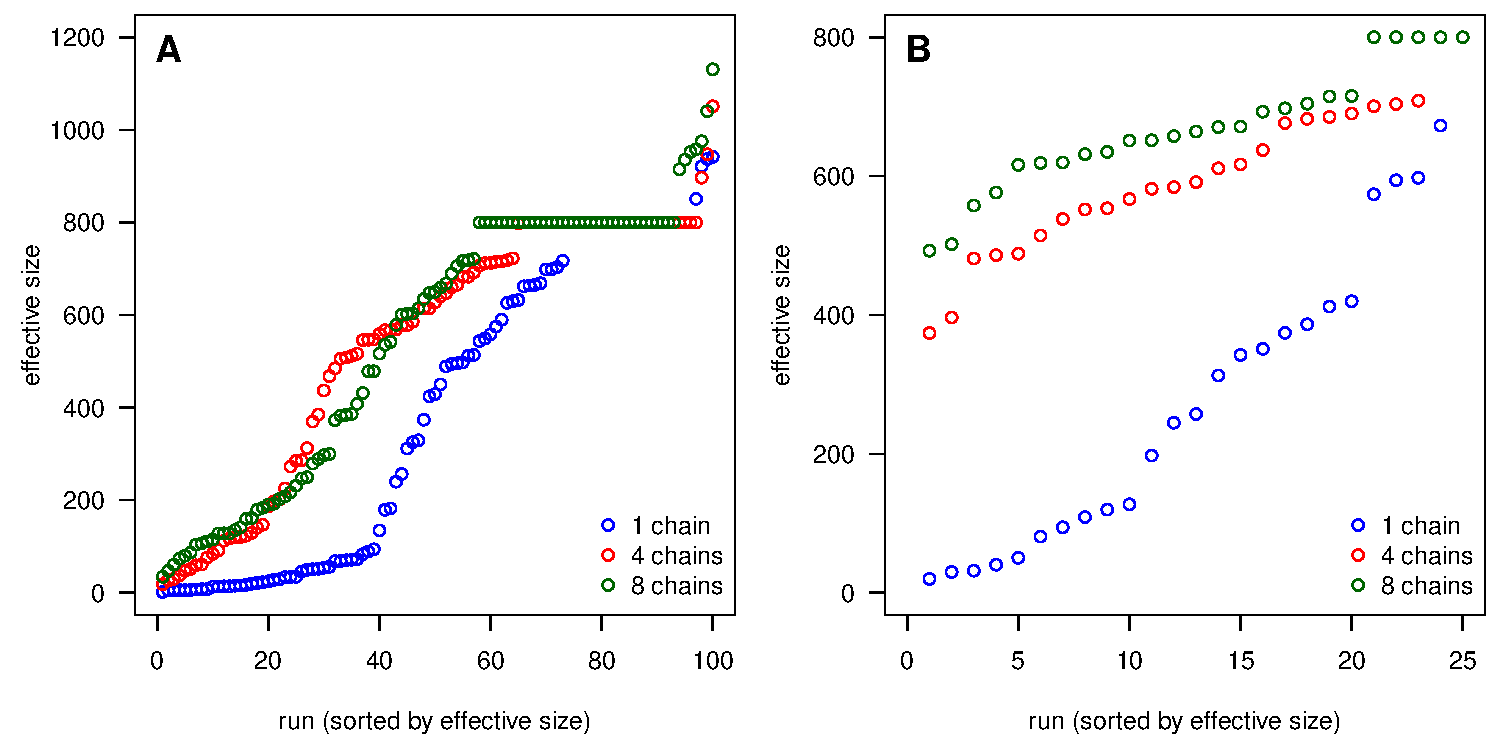
\includegraphics[width=14cm]{eff-size.pdf}
\end{center}
\caption{Effective sizes of the log-likelihood for
    (A) runs of 100 simulated trees and (B) 25 runs of the skink tree.
    Runs are sorted by their effective size.}
\label{fig:eff-size}
\end{figure}


For the simulated trees,
we found that the difference in the coefficient of variation
between runs with one chain and runs with four chains
overlapped zero 52.6\% of the time.
%
For runs with one and eight chains,
this difference overlapped 51.8\% of the time.
%
These results suggest that there was no difference
in convergence between runs with and without \MCMCMC\ in simulated trees.
%
For the skink tree, however,
the difference in the coefficient of variation
between runs with one chain and runs with four chains
overlapped with zero only 4.7\% of the time.
%
For runs with one and eight chains,
this difference overlapped 26.2\% of the time.
%
This result suggests that runs with \MCMCMC\ 
converged better than those without it in the skink tree.


We found that the parallellism of \MCMCMCMC\ 
reduced the amount of time runs would have taken without it.
%
For the simulated trees, which ran for 25 million generations,
the mean number of hours that runs took with
one chain, four chains, and eight chains were
6.3, 6.5, and 6.8 hr.
%
Without \MCMCMCMC, the runs with four and eight chains
would have taken 25.2 and 50.4 hr.
%
For the skink tree, which ran for 100 million generations,
the means were 18.8, 20.7, and 21.4 hr for one, four, and eight chains.
%
Without \MCMCMCMC, the runs with four and eight chains
would have taken 75.2 (3.1 d) and 150.5 hr (6.3 d).


% Point out the importance of the results and place them in the context
% of previous studies and in relation to the application of the work
% (expanding on the Synthesis and applications section of the Summary).
% Where appropriate, set out recommendations for management or policy
\section*{Discussion}

The discussion will go here.


\section*{Acknowledgements}

This research was supported in part through computational resources
and services provided by Advanced Research Computing
at the University of Michigan, Ann Arbor.


\bibliography{mc3}

\end{document}
